\documentclass[11pt,a4paper]{article}
\usepackage[utf8]{inputenc}
\usepackage{lmodern} % Must precede fontenc: the EC fonts may not be installed
\usepackage[T1]{fontenc}
\usepackage[margin=2.5cm]{geometry}
\usepackage{amsmath}
\usepackage{graphicx}
\usepackage{booktabs}
\usepackage{caption}

% Polish hyphenation is optional, so the report also compiles on TeX installations without it.
\IfFileExists{polish.ldf}{%
  \usepackage[polish]{babel}%
}{%
  \hyphenpenalty=10000
  \exhyphenpenalty=10000
  \emergencystretch=3em
  \renewcommand{\figurename}{Rysunek}
  \renewcommand{\tablename}{Tabela}
}

\title{Biosygnały, laboratorium 5--6:\\beztrendowa analiza fluktuacji (DFA)}
\author{Dominik Zawlocki}
\date{19 listopada 2026}

\begin{document}
\maketitle

\section{Cel i dane}
Celem ćwiczenia było zaimplementowanie beztrendowej analizy fluktuacji (DFA) i~wyznaczenie współczynników skalowania $\alpha_1$ (krótkoterminowego) oraz $\alpha_2$ (długoterminowego) dla zapisów odstępów RR. Analizę przeprowadzono najpierw dla dwóch pojedynczych zapisów:
\begin{itemize}
  \item \textbf{nsr001}: osoba zdrowa (kobieta, 64 lata), rytm zatokowy, 106\,460 odstępów RR, 22,5~h zapisu,
  \item \textbf{chf206}: pacjentka z~niewydolnością serca (38 lat, NYHA~III), 135\,470 odstępów RR, 20,9~h zapisu.
\end{itemize}
Następnie wyznaczono współczynniki dla wszystkich rekordów baz Physionet: Normal Sinus Rhythm RR Interval Database (NSR2DB, 54 rekordy) oraz Congestive Heart Failure RR Interval Database (CHF2DB, 29 rekordów).

\section{Metoda}
\subsection{Przygotowanie danych}
Czasy uderzeń $t_k$ wyznaczono jako sumę skumulowaną odstępów RR. Następnie odrzucono odstępy spoza zakresu fizjologicznego 0,3--2~s (HR 30--200~bpm): 3 dla nsr001 i~28 dla chf206. Sumę liczono przed filtracją, aby usunięcie odstępu nie przesuwało kolejnych uderzeń na osi czasu. Pobudzeń ektopowych nie usuwano.

\subsection{Algorytm DFA}
Dla przefiltrowanego ciągu odstępów $x(i)$, $i = 1, \dots, L$, wykonano kolejne kroki algorytmu.
\begin{enumerate}
  \item Całkowanie sygnału względem wartości średniej:
  \begin{equation}
    y(k) = \sum_{i=1}^{k} \big(x(i) - x_{\mathrm{mean}}\big).
  \end{equation}
  \item Podział na $L/n$ rozłącznych okien o~długości $n$ uderzeń. Wykorzystywano pierwsze $N = \lfloor L/n \rfloor \cdot n$ próbek, a~pozostałe (mniej niż $n$) pomijano.
  \item Dopasowanie w~każdym oknie prostej $y_n(k)$ metodą najmniejszych kwadratów. Jako zmienną niezależną przyjęto czas uderzenia $t_k$, tak jak na rys.~1 w~instrukcji. Dzięki temu przerwy po usuniętych artefaktach są uwzględnione na osi czasu.
  \item Obliczenie średniej kwadratowej fluktuacji wokół trendu:
  \begin{equation}
    F(n) = \sqrt{\frac{1}{N} \sum_{k=1}^{N} \big[y(k) - y_n(k)\big]^2}.
  \end{equation}
  \item Wyznaczenie $\alpha_1$ i~$\alpha_2$ jako nachyleń prostych dopasowanych metodą najmniejszych kwadratów do zależności $\log_{10} F(n)$ od $\log_{10} n$, odpowiednio dla $4 \le n \le 16$ i~$16 < n \le 64$.
\end{enumerate}

Funkcja \texttt{dfa} (plik \texttt{DFA.py}) wykonuje wszystkie kroki dla $n = 4, \dots, 64$ i~zwraca $F(n)$, $\alpha_1$, $\alpha_2$ oraz wartości $\log_{10} n$ i~$\log_{10} F(n)$.

Trendy lokalne liczone są dla wszystkich okien jednocześnie. Sygnał układany jest w~macierz o~wierszach będących kolejnymi oknami, w~każdym oknie od $t_k$ i~$y(k)$ odejmowane są ich średnie ($\tilde t_k$, $\tilde y_k$), a~nachylenie prostej wynosi wtedy
\begin{equation}
  a = \frac{\sum_k \tilde t_k \, \tilde y_k}{\sum_k \tilde t_k^2},
\end{equation}
przy zerowym wyrazie wolnym. Centrowanie poprawia też uwarunkowanie numeryczne, bo czasy $t_k$ sięgają $10^5$~s, a~okno trwa kilka sekund.

\section{Etapy algorytmu}
Rys.~\ref{fig:rr-nsr} i~\ref{fig:rr-chf} pokazują interwały RR i~sygnał scałkowany $y(k)$. Sygnał $y(k)$ rośnie, gdy rytm jest wolniejszy od średniej, i~maleje, gdy szybszy. Dla nsr001 widać wyraźny podział na dzień i~noc (dłuższe odstępy RR w~godzinach 9--20 zapisu). Dla chf206 odstępy RR są krótsze i~znacznie mniej zmienne (SD 48~ms wobec 169~ms), choć występuje wiele pojedynczych odstępów odbiegających od reszty.

Rys.~\ref{fig:trends-nsr} i~\ref{fig:trends-chf} pokazują proste dopasowane w~oknach o~długości $n = 4$, 16 i~32 na fragmencie 64 uderzeń ze środka zapisu. Dla czytelności od $y(k)$ odjęto prostą łączącą końce fragmentu. Jest to przekształcenie liniowe, więc dopasowane proste pozostają prostymi najmniejszych kwadratów. Dla małego $n$ trend nadąża za sygnałem, a~wraz ze wzrostem $n$ odchylenia od trendu rosną. Przyrost $F(n)$ z~$n$ opisują właśnie współczynniki $\alpha$. W~fragmencie chf206 widać pod koniec nieregularne uderzenia, które dają duże odchylenia już dla najmniejszych okien.

\begin{figure}[p]
  \centering
  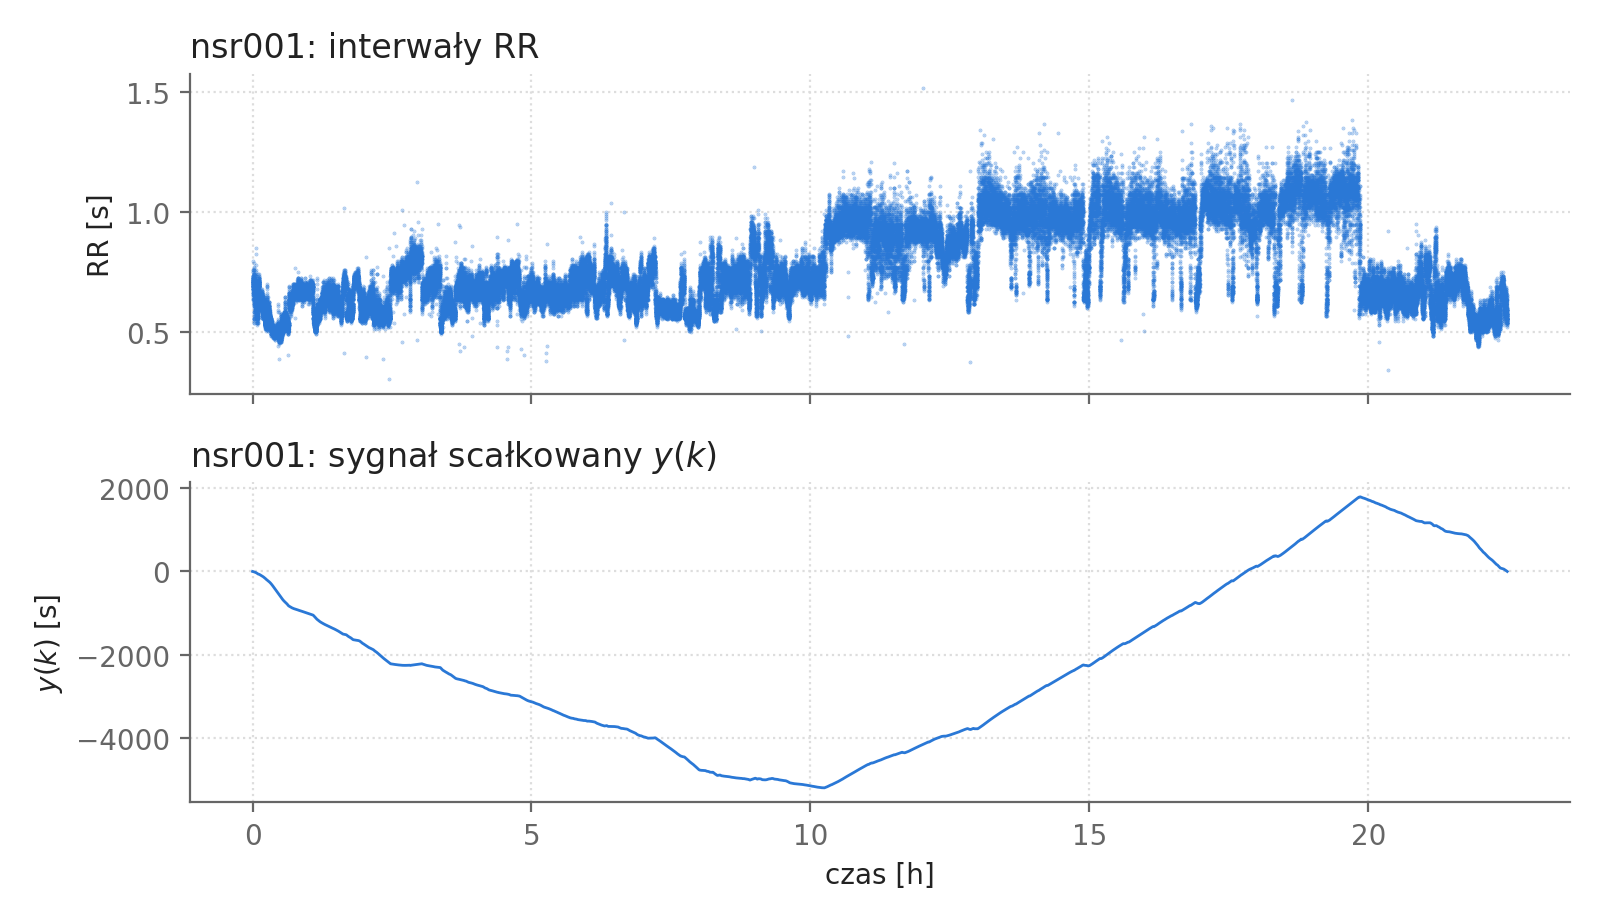
\includegraphics[width=0.92\textwidth]{figures/rr_int_nsr001.png}
  \caption{nsr001: interwały RR (u~góry) i~sygnał scałkowany $y(k)$ (na dole).}
  \label{fig:rr-nsr}

  \vspace{4mm}
  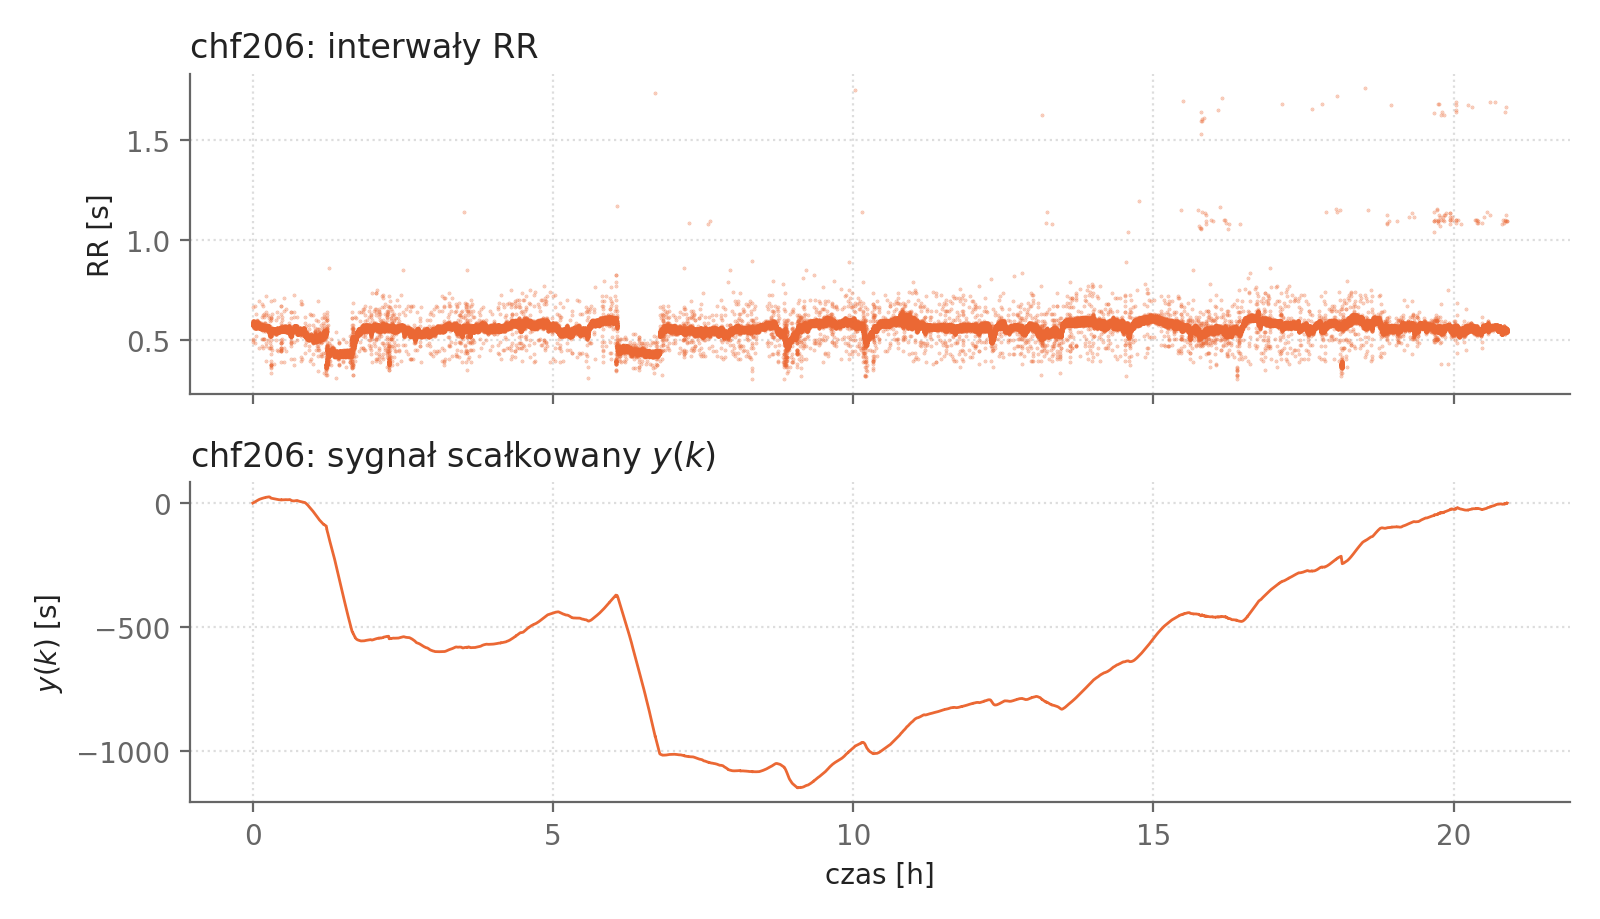
\includegraphics[width=0.92\textwidth]{figures/rr_int_chf206.png}
  \caption{chf206: interwały RR (u~góry) i~sygnał scałkowany $y(k)$ (na dole).}
  \label{fig:rr-chf}
\end{figure}

\begin{figure}[p]
  \centering
  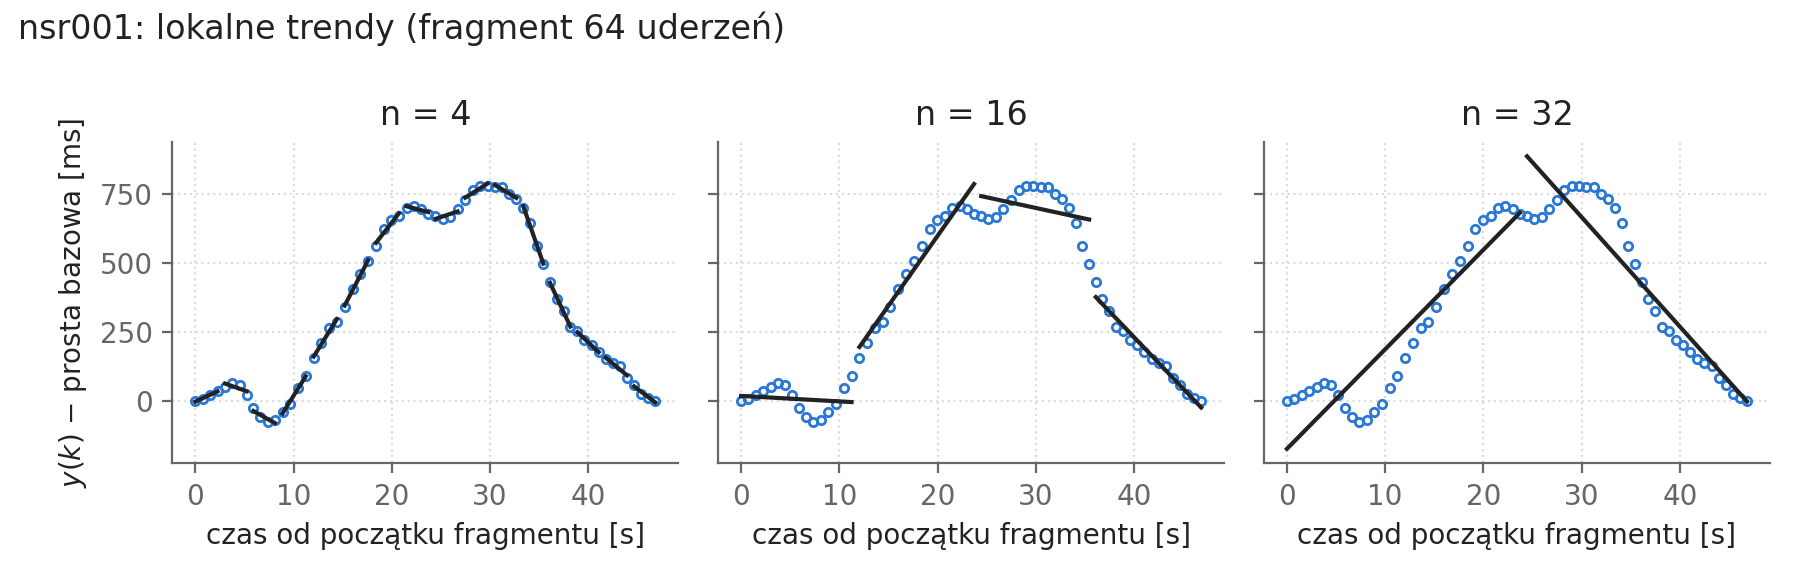
\includegraphics[width=\textwidth]{figures/trends_nsr001.png}
  \caption{nsr001: trendy lokalne dla $n = 4$, 16 i~32 na fragmencie 64 uderzeń. Od $y(k)$ odjęto prostą łączącą końce fragmentu.}
  \label{fig:trends-nsr}

  \vspace{4mm}
  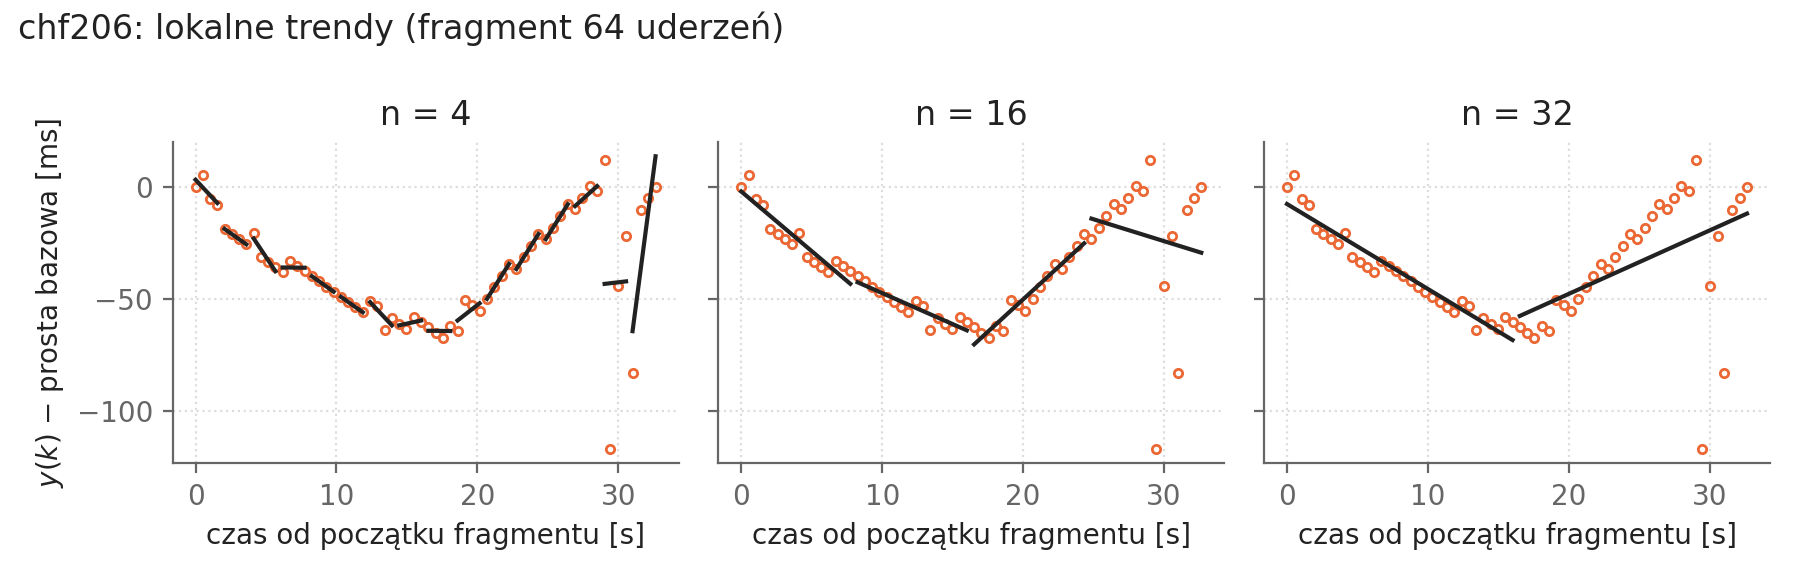
\includegraphics[width=\textwidth]{figures/trends_chf206.png}
  \caption{chf206: trendy lokalne dla $n = 4$, 16 i~32 na fragmencie 64 uderzeń. Od $y(k)$ odjęto prostą łączącą końce fragmentu.}
  \label{fig:trends-chf}
\end{figure}

\section{Wyniki dla nsr001 i chf206}
Zależność $\log_{10} F(n)$ od $\log_{10} n$ pokazano na rys.~\ref{fig:logF}, a~wyznaczone współczynniki zebrano w~tab.~\ref{tab:alpha}. W~obu zakresach punkty dobrze układają się na prostych, więc opis za pomocą dwóch współczynników jest uzasadniony.

\begin{figure}[ht]
  \centering
  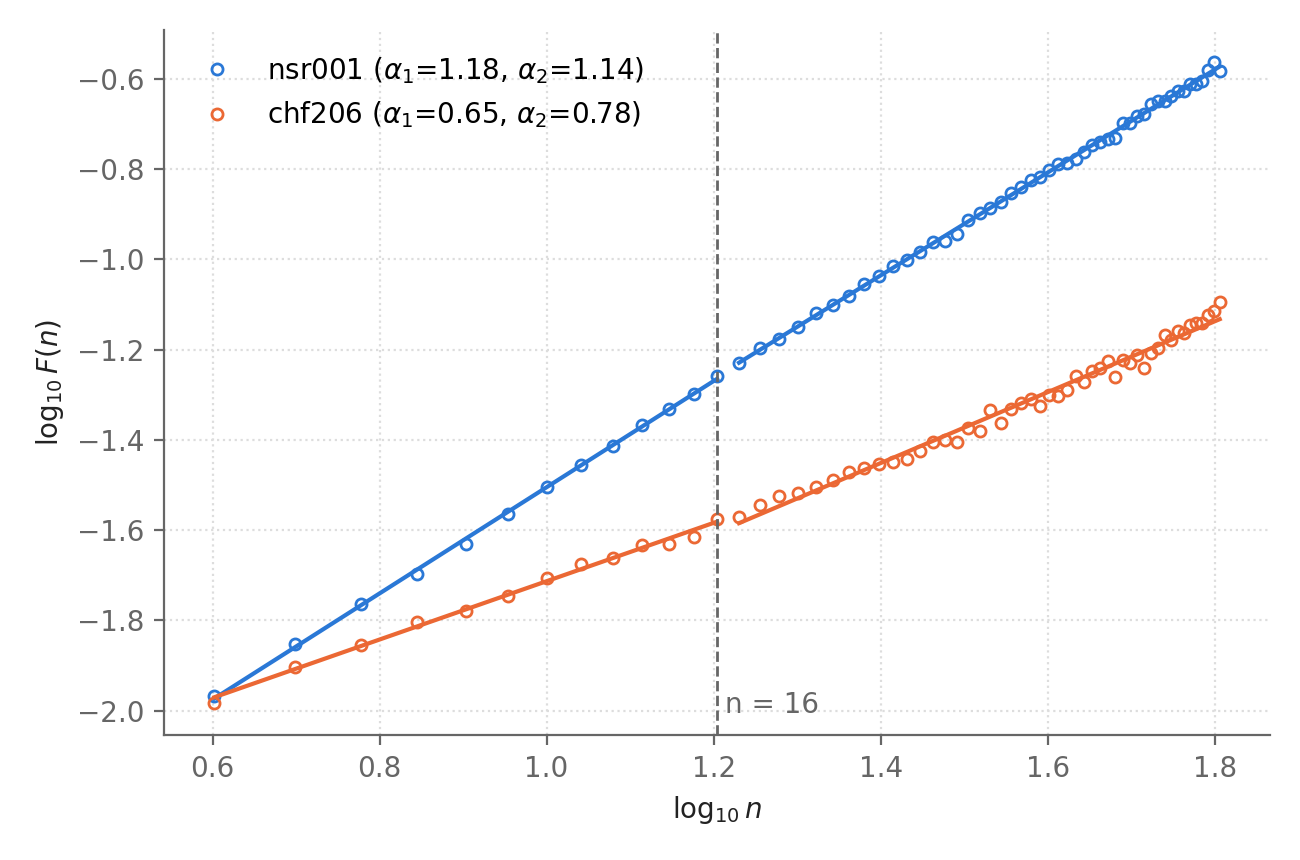
\includegraphics[width=0.8\textwidth]{figures/logF_nsr001_chf206.png}
  \caption{$\log_{10} F(n)$ w~funkcji $\log_{10} n$ dla nsr001 i~chf206 wraz z~prostymi dopasowanymi w~zakresach $n \le 16$ i~$n > 16$.}
  \label{fig:logF}
\end{figure}

\begin{table}[ht]
  \centering
  \caption{Statystyki odstępów RR i~współczynniki DFA dla nsr001 i~chf206.}
  \label{tab:alpha}
  \begin{tabular}{lrrrrr}
    \toprule
    Sygnał & średni RR [s] & HR [bpm] & SD RR [ms] & $\alpha_1$ & $\alpha_2$ \\
    \midrule
    nsr001 & 0,760 & 78,9 & 168,6 & 1,176 & 1,140 \\
    chf206 & 0,555 & 108,2 & 48,1 & 0,646 & 0,785 \\
    \bottomrule
  \end{tabular}
\end{table}

\paragraph{Porównanie.}
\begin{itemize}
  \item \textbf{Poziom fluktuacji:} $F(n)$ dla chf206 jest mniejsze we wszystkich skalach, co odpowiada mniejszej zmienności rytmu (SD RR około 3,5-krotnie mniejsze).
  \item \textbf{$\alpha_1$:} dla nsr001 wynosi 1,18, czyli blisko wartości 1 charakterystycznej dla szumu typu $1/f$. Oznacza to silne korelacje krótkoterminowe, typowe dla zdrowej regulacji rytmu, w~której istotny udział ma modulacja oddechowa i~baroreceptorowa. Dla chf206 $\alpha_1 = 0{,}65$ jest bliskie wartości 0,5, którą daje nieskorelowany szum biały. Krótkoterminowa dynamika rytmu jest więc znacznie bardziej przypadkowa. Obniżenie $\alpha_1$ w~niewydolności serca jest zgodne z~literaturą (Peng i~in., 1995).
  \item \textbf{$\alpha_2$:} wartości są bliższe sobie (1,14 i~0,79), ale dla chf206 również niższe. Korelacje długoterminowe są w~CHF osłabione, choć w~mniejszym stopniu niż krótkoterminowe.
  \item \textbf{Zmiana nachylenia:} dla nsr001 $\alpha_1$ jest nieco większe od $\alpha_2$, a~dla chf206 odwrotnie ($\alpha_1 < \alpha_2$). W~CHF to w~krótkich skalach rytm najbardziej traci strukturę korelacyjną.
\end{itemize}

Zapis chf206 zawiera dużo pobudzeń pozazatokowych: według adnotacji 9748 pobudzeń przedsionkowych (A) i~1346 komorowych (V), czyli około 8\% wszystkich uderzeń, wobec 81 w~nsr001. Pobudzenia te dodają do sygnału składową o~charakterze szumu białego i~mogą dodatkowo obniżać $\alpha_1$. Obniżenie $\alpha_1$ wynika więc zarówno ze zmian w~autonomicznej regulacji rytmu, jak i~z~zaburzeń rytmu. Nie da się tych przyczyn rozdzielić bez usunięcia pobudzeń ektopowych.

\section{Analiza baz NSR2DB i CHF2DB}
Rekordy wczytano z~plików adnotacji \texttt{.ecg} za pomocą pakietu \texttt{wfdb}. Odstępy RR obliczono jako różnice chwil kolejnych uderzeń podzielone przez częstotliwość próbkowania adnotacji (128~Hz). Pominięto adnotacje niebędące uderzeniami (np. \texttt{\textasciitilde}, oznaczające zakłócenia). Dla nsr001 tak uzyskane odstępy zgadzają się z~plikiem używanym w~poprzednich punktach z~dokładnością do 0,5~ms (zaokrąglenie do milisekund). Na każdym rekordzie wykonano ten sam algorytm co wcześniej, łącznie z~filtracją odstępów niefizjologicznych.

\begin{table}[ht]
  \centering
  \caption{Podsumowanie baz i~statystyki współczynników DFA (średnia $\pm$ odchylenie standardowe, mediana, zakres).}
  \label{tab:db}
  \begin{tabular}{lrrrrr}
    \toprule
    Baza & rekordy & odstępy RR & usunięte & $\alpha_1$ & $\alpha_2$ \\
    \midrule
    NSR2DB & 54 & 5\,790\,450 & 0,18\% & $1{,}17 \pm 0{,}21$ & $1{,}00 \pm 0{,}10$ \\
           &    &             &        & 1,23 (0,42--1,44) & 1,00 (0,80--1,27) \\
    \midrule
    CHF2DB & 29 & 3\,312\,166 & 0,18\% & $0{,}70 \pm 0{,}26$ & $0{,}90 \pm 0{,}22$ \\
           &    &             &        & 0,66 (0,21--1,29) & 0,87 (0,56--1,34) \\
    \bottomrule
  \end{tabular}
\end{table}

Statystyki zebrano w~tab.~\ref{tab:db}, rekordy na płaszczyźnie cech $(\alpha_1, \alpha_2)$ pokazano na rys.~\ref{fig:plane}, a~wartości dla poszczególnych rekordów podano w~załączniku. Zapisy trwają od 21,2 do 24,1~h w~NSR2DB i~od 17,0 do 24,0~h w~CHF2DB. Średnie wartości dla baz potwierdzają obserwacje z~pojedynczych zapisów: w~CHF2DB oba współczynniki są niższe, przy czym różnica jest znacznie większa dla $\alpha_1$. Rozrzut obu współczynników jest w~CHF2DB większy niż w~NSR2DB, szczególnie dla $\alpha_2$ (odchylenie standardowe 0,22 wobec 0,10).

Współczynniki zależą w~niewielkim stopniu od ułożenia okien. Rekord chf206 wczytany z~bazy daje $\alpha_1 = 0{,}659$ i~$\alpha_2 = 0{,}790$, a~plik użyty w~poprzednich punktach $0{,}646$ i~$0{,}785$. Pliki różnią się tylko dodatkowym pierwszym odstępem, który przesuwa podział na okna o~jedno uderzenie. Przesunięcie początku o~1--3 uderzenia zmienia $\alpha_1$ dla tego rekordu o~mniej niż 0,01, więc różnice tej wielkości między rekordami nie są istotne.

\begin{figure}[ht]
  \centering
  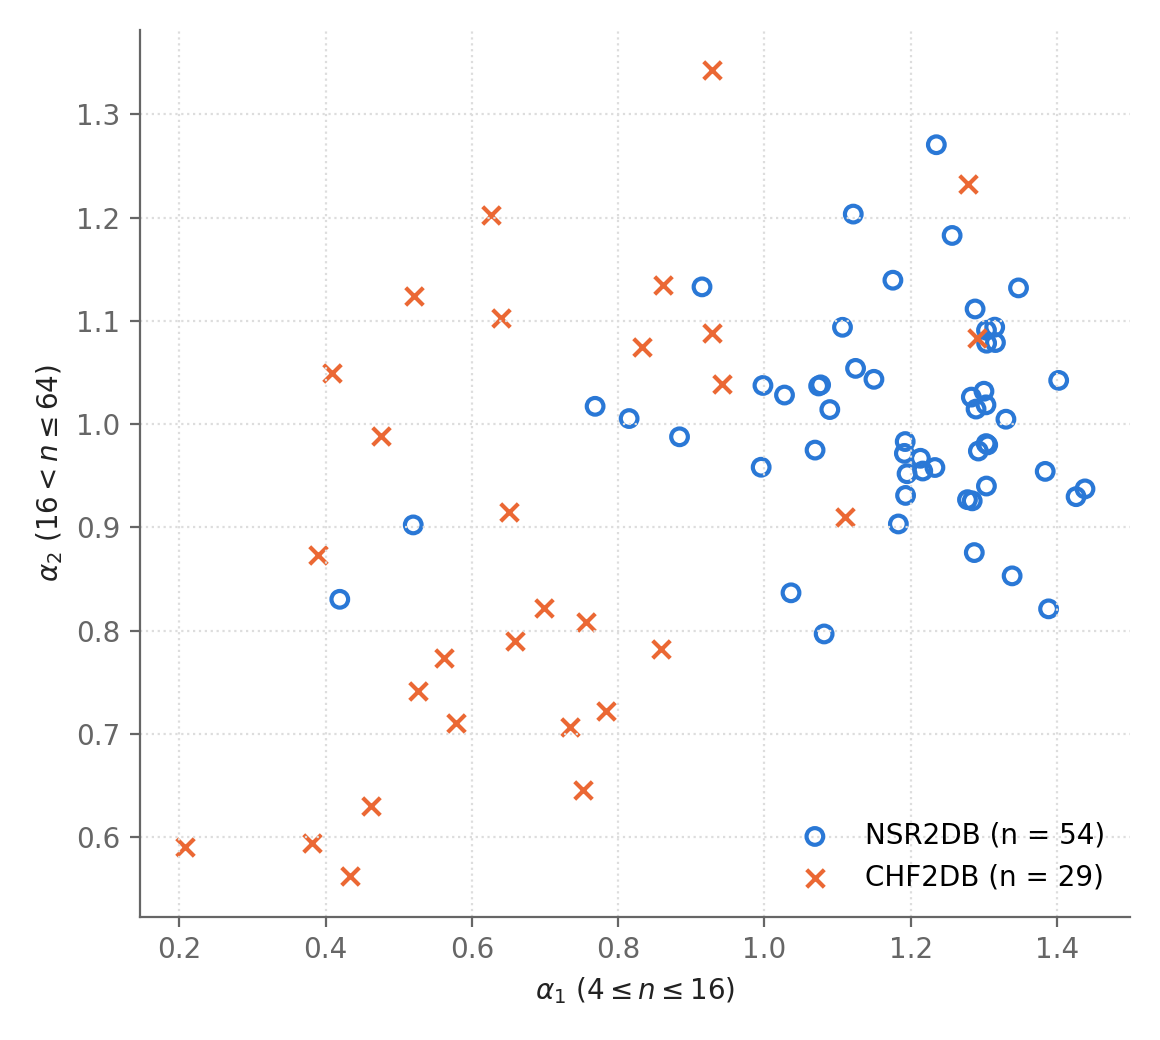
\includegraphics[width=0.62\textwidth]{figures/alpha_plane.png}
  \caption{Rekordy baz NSR2DB (kółka) i~CHF2DB (krzyżyki) na płaszczyźnie cech DFA $(\alpha_1, \alpha_2)$.}
  \label{fig:plane}
\end{figure}

\section{Wnioski}
DFA pozwala opisać dynamikę rytmu serca dwoma liczbami, które charakteryzują korelacje odstępów RR w~krótkich ($n \le 16$) i~długich ($n > 16$) skalach, niezależnie od trendów wolnozmiennych. U~osoby zdrowej $\alpha_1 \approx 1{,}2$, co oznacza silnie skorelowaną, złożoną regulację rytmu. U~pacjentki z~niewydolnością serca $\alpha_1$ spada do około 0,65, a~krótkoterminowa dynamika rytmu zbliża się do nieskorelowanego szumu. Ten sam kierunek zmian widać w~średnich dla całych baz NSR2DB i~CHF2DB.

Ograniczenia: pobudzenia ektopowe nie zostały usunięte, a~ich udział jest znacznie większy w~zapisach CHF. Zapisy obejmują dobę, łącząc okresy snu i~czuwania o~różnej dynamice. Grupy różnią się składem: w~NSR2DB wiek wynosi 28,5--76 lat (mediana 65), a~w~CHF2DB 34--79 lat (mediana 58). Płeć podano dla wszystkich osób z~NSR2DB, ale tylko dla 10 z~29 pacjentów CHF2DB. Pacjenci CHF2DB mają różne stadia choroby (NYHA~I: 4, II: 8, III: 17). Różnic nie można więc przypisywać wyłącznie niewydolności serca.

\appendix
\section{Współczynniki DFA dla wszystkich rekordów}
\begin{table}[ht]
  \centering
  \small
  \caption{Współczynniki DFA dla rekordów bazy NSR2DB.}
  \label{tab:nsr-all}
  \begin{tabular}{lrr|lrr|lrr}
  \toprule
  Rekord & $\alpha_1$ & $\alpha_2$ & Rekord & $\alpha_1$ & $\alpha_2$ & Rekord & $\alpha_1$ & $\alpha_2$ \\
  \midrule
  nsr001 & 1,18 & 1,14 & nsr019 & 1,29 & 1,11 & nsr037 & 1,30 & 1,09 \\
  nsr002 & 1,11 & 1,09 & nsr020 & 1,28 & 0,93 & nsr038 & 1,39 & 0,82 \\
  nsr003 & 0,88 & 0,99 & nsr021 & 1,26 & 1,18 & nsr039 & 1,22 & 0,95 \\
  nsr004 & 1,28 & 1,03 & nsr022 & 1,08 & 1,04 & nsr040 & 0,91 & 1,13 \\
  nsr005 & 1,09 & 1,01 & nsr023 & 1,12 & 1,20 & nsr041 & 1,19 & 0,93 \\
  nsr006 & 1,29 & 0,97 & nsr024 & 0,52 & 0,90 & nsr042 & 1,30 & 1,08 \\
  nsr007 & 1,15 & 1,04 & nsr025 & 1,04 & 0,84 & nsr043 & 1,19 & 0,98 \\
  nsr008 & 1,30 & 1,02 & nsr026 & 1,24 & 1,27 & nsr044 & 0,42 & 0,83 \\
  nsr009 & 1,29 & 0,88 & nsr027 & 1,38 & 0,95 & nsr045 & 1,18 & 0,90 \\
  nsr010 & 1,23 & 0,96 & nsr028 & 1,29 & 1,01 & nsr046 & 1,03 & 1,03 \\
  nsr011 & 1,07 & 1,04 & nsr029 & 1,43 & 0,93 & nsr047 & 1,32 & 1,08 \\
  nsr012 & 1,32 & 1,09 & nsr030 & 1,31 & 0,98 & nsr048 & 1,44 & 0,94 \\
  nsr013 & 1,30 & 0,98 & nsr031 & 1,34 & 0,85 & nsr049 & 1,08 & 0,80 \\
  nsr014 & 0,77 & 1,02 & nsr032 & 1,00 & 1,04 & nsr050 & 1,19 & 0,97 \\
  nsr015 & 1,28 & 0,93 & nsr033 & 1,33 & 1,00 & nsr051 & 1,12 & 1,05 \\
  nsr016 & 1,21 & 0,97 & nsr034 & 1,40 & 1,04 & nsr052 & 1,35 & 1,13 \\
  nsr017 & 0,82 & 1,01 & nsr035 & 1,20 & 0,95 & nsr053 & 1,30 & 1,03 \\
  nsr018 & 1,00 & 0,96 & nsr036 & 1,07 & 0,97 & nsr054 & 1,30 & 0,94 \\
  \bottomrule
  \end{tabular}
\end{table}

\begin{table}[ht]
  \centering
  \small
  \caption{Współczynniki DFA dla rekordów bazy CHF2DB.}
  \label{tab:chf-all}
  \begin{tabular}{lrr|lrr|lrr}
  \toprule
  Rekord & $\alpha_1$ & $\alpha_2$ & Rekord & $\alpha_1$ & $\alpha_2$ & Rekord & $\alpha_1$ & $\alpha_2$ \\
  \midrule
  chf201 & 1,28 & 1,23 & chf211 & 1,11 & 0,91 & chf221 & 0,65 & 0,92 \\
  chf202 & 0,93 & 1,09 & chf212 & 0,75 & 0,65 & chf222 & 0,70 & 0,82 \\
  chf203 & 0,63 & 1,20 & chf213 & 0,56 & 0,77 & chf223 & 0,53 & 0,74 \\
  chf204 & 0,52 & 1,12 & chf214 & 0,38 & 0,59 & chf224 & 0,86 & 1,14 \\
  chf205 & 0,73 & 0,71 & chf215 & 0,21 & 0,59 & chf225 & 0,78 & 0,72 \\
  chf206 & 0,66 & 0,79 & chf216 & 0,94 & 1,04 & chf226 & 0,39 & 0,87 \\
  chf207 & 0,43 & 0,56 & chf217 & 0,83 & 1,07 & chf227 & 0,46 & 0,63 \\
  chf208 & 0,58 & 0,71 & chf218 & 0,76 & 0,81 & chf228 & 0,64 & 1,10 \\
  chf209 & 0,48 & 0,99 & chf219 & 1,29 & 1,08 & chf229 & 0,86 & 0,78 \\
  chf210 & 0,41 & 1,05 & chf220 & 0,93 & 1,34 &  & &  \\
  \bottomrule
  \end{tabular}
\end{table}

\end{document}
